\begin{flushright} {\tiny {\color{gray} (tikz\_tetrahedron.tex)}} \end{flushright}
%~~~~~~~~~~~~~~~~~~~~~~~~~~~~~~~~~~~~~~~~~~~~~~~~~~~~~~~~~~~~~~~~~~~~~~~~~~~~~~~~~~~~~~~~~~~~~~~~~~
\begin{center}
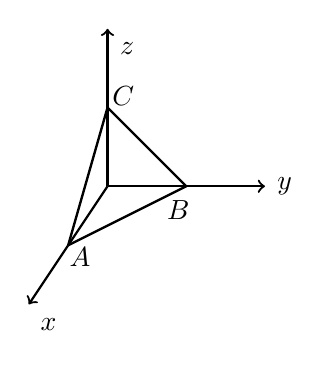
\begin{tikzpicture}
%\draw[step=0.5cm,gray,very thin] (0,0) grid (4,4); %background grid

\draw [thick,->] (1.5,2) -- (3.5,2);
\draw [thick,->] (1.5,2) -- (1.5,4);
\draw [thick,->] (1.5,2) -- (0.5,0.5);

\node[] at (0.75,0.25) {$x$};
\node[] at (3.75,2) {$y$};
\node[] at (1.75,3.75) {$z$};

\draw[line width=0.3mm] (1,1.25) -- (2.5,2) ;   
\node[] at (2.4,1.7) {$B$};

\draw[line width=0.3mm] (2.5,2) -- (1.5,3) ;   
\node[] at (1.7,3.15) {$C$};

\draw[line width=0.3mm] (1.5,3) -- (1,1.25) ;   
\node[] at (1.15,1.1) {$A$};

\end{tikzpicture}
\end{center}
